%--------------------------------
%	Paquetes y configuraciones 
%--------------------------------

\documentclass[a4paper,12pt]{article}
\usepackage[utf8x]{inputenc}
\usepackage[spanish]{babel}
\usepackage{amsmath}
\usepackage{graphicx}
%\usepackage{showframe}
\usepackage[margin=1in]{geometry}
\usepackage{empheq}
\usepackage[most]{tcolorbox}
\usepackage{pgfplots}
\pgfplotsset{compat=newest}
\usepgfplotslibrary{patchplots}

\newtcbox{\mymath}[1][]{
    nobeforeafter, math upper, tcbox raise base,
    enhanced, colframe=blue!30!black,
    colback=blue!30, boxrule=1pt,#1}


%\PassOptionsToPackage{svgnames}{xcolor}
%\usepackage{lipsum}
\tcbuselibrary{skins,breakable}
%\usetikzlibrary{shadings,shadows}

%\newenvironment{block}[1]{%
%    \tcolorbox[beamer,%
%    noparskip,breakable,
%    title=#1]}%
%    {\endtcolorbox}

%----------------------------
%   Comienzo del documento
%----------------------------

\begin{document}
    %\sffamily % Fuente sans serif
    \newcommand{\HRule}{\rule{\linewidth}{0.5mm}}
    
    %-----------------
    %   Portada
    %-----------------
    
    \begin{titlepage}
        \center

        %
\includegraphics[scale=0.15]{logo.png}\\[1cm] % Descomentar para usar el logo del JVG
        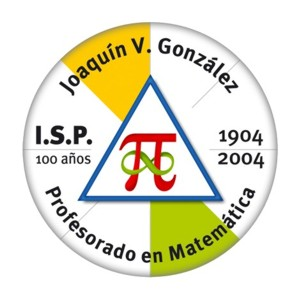
\includegraphics[scale=0.4]{pinmatematica.jpg}\\[1cm]
        \textsc{\Large Instituto Superior del Profesorado}\\[0.3cm]
        \textsc{\LARGE Dr. Joaquín V. González}\\[1cm]
        \textsc{\large Profesorado de Educación Superior en Matemática}\\[0.5cm]
        
        \HRule \\[0.4cm]
            {\huge \bfseries Historia de la Matemática}\\[0.3cm]
            \Large Apuntes de Clase\\
            \large Cursada del año 2019\\
        \HRule \\[1.5cm]
        
        \begin{minipage}{0.4\textwidth}
            \begin{flushleft} 
                \large
                \emph{Creado por:}\\
                Javier Spina
                javierspina@gmail.com
            \end{flushleft}
        \end{minipage}
        ~
        \begin{minipage}{0.4\textwidth}
            \begin{flushright} 
                \large
                \emph{Docente:}\\
                Cecilia Crespo Crespo
            \end{flushright}
        \end{minipage}\\[3cm]
        
        \vfill
        {\large \today}
        
        \restoregeometry
    \end{titlepage}

\tableofcontents
\pagebreak

%-------------------------%
%-----Document Setup------%
%-------------------------%
\documentclass[a4paper,12pt,openany]{article}
\usepackage[utf8x]{inputenc}
\usepackage[spanish]{babel}
\usepackage[left=3cm, right=2cm, top=2.5cm, bottom=3cm]{geometry}
%\usepackage{savetrees}
\usepackage{verbatim}
\linespread{1.6}
%\setlength{\footskip}{20pt}
\usepackage{graphicx}


%-------------------------%
%------Document Code------%
%-------------------------%
\newcommand{\thought}[1]{\textit{#1}}

\newcommand{\scenechange}{
  \par
  \vspace{\baselineskip}
  \par
\noindent}
%Creates a line break for a change of scene

\newcommand{\majorchange}{
  \par
  \vspace{\baselineskip}
  \hfill
  \textasteriskcentered
  \hfill
  \vspace{\baselineskip}
\noindent}
%creates a major line break, split by an asterisk for scene changes at the end of a page of where a sense of a major change is required. 

%-------------------------%
%------Main Document------%
%-------------------------%
\begin{document}
%\title{China}
%\date{}
%\maketitle
\section*{China}
\subsection*{Cultura y sociedad}
Las culturas previas a Grecia eran empíricas. En la cultura griega hay un cambio de paradigma sobre qué es la ciencia y qué es la matemática, en ese cambio pasamos a dejar de tener lo que se llaman explicaciones míticas de los fenómenos y se pasa a tener explicaciones racionales. El griego busca explicar la realidad y todo lo que los rodea a través de la razón. Para los griegos, la razón es la que va a regir todo tipo de conocimiento y se va a constituir como algo característico del ser humano. 

A diferencia de otras culturas donde se buscaban resultados por ensayo y error, los griegos apuntan a generar una sistematización de conocimientos, una generalización de resultados. Buscan propiedades atribuibles a un conjunto en vez de ir por los casos particulares. Aparecen las demostraciones deductivas, una vez efectuada la demostración se va a saber para qué casos aplica.

Se distinguen tres períodos

\begin{enumerate}[topsep=0pt,itemsep=-1ex,partopsep=1ex,parsep=1ex]
    \item Clásico o Helénico: surgimiento del pensamiento racional (600 a.C. - 300 a.C.)
    \item Helenístico o Alejandrino: apogeo (300 a.C. - 300 d.C.)
    \item Grecorromano: decadencia (300 d.C. - 600 d.C.)
\end{enumerate}
%add additional sections by creating new section#.tex files and copying the two lines above. You can number sections (remove the asterisks) or name them (in the curly braces) or even use chapters instead. Ooo, and don't forget you can do parts too!

\subsection*{Filosofía}
En el período helénico se sientan las bases del pensamiento griego. Surgen los llamados pensadores presocráticos, que buscan el principio de todas las cosas, en el intento de la explicación racional, el llamado arjé. A partir de esta búsqueda es que dan explicaciones de los distintos fenómenos que encuentran. Thales de Mileto y Pitágoras de Samos son de este período.

\subsection*{Matemática y sus aplicaciones}
Para Thales, el arjé es el agua, dice que cualquier cosa del universo está compuesta de agua. A Thales se le atribuyen las primeras demostraciones racionales, esas demostraciones donde se enuncia un teorema y se trata de demostrarlo con el pensamiento deductivo. Sin embargo, en algunas de sus demostraciones incurren en lo que se denominan demostraciones circulares. Es decir, que para demostrar una propiedad B utiliza una propiedad A y para demostrar A vuelve a utilizar B.

Algo que le dio mucho prestigio a Thales fue haber predecido el primer eclipse. En su búsqueda de tratar de explicar fenómenos, empezó a tener un modelo del movimiento del Sol, la Tierra y la Luna. Luego logró explicar un eclipse de Sol, diciendo que la Luna se ubica entre la Tierra y el Sol, además de poder predecirlo para el 28 de mayo del 585 a.C.. Esta predicción fue afamada y le dió prestigio porque el eclipse se dió durante una batalla contra los macedonios: el enemigo quedó confundido por el fenómeno, pero los griegos al saber del rumor, pudieron no distraerse tanto y así derrotaron a los macedonios fácilmente. La credibilidad que ganó Thales permitió que su modelo astronómico sea respetado. Fue incluido en varios listados de siete sabios griegos (de hecho, fue el único presente en todos los listados).

Otro modelo que tiene Thales es de los imanes. Él explica que dentro de un imán hay unos pequeños imanes. Por ejemplo con el fenómeno de la imantación del hierro: dentro de este material los pequeños imanes están desordenados, pero al estar en contacto con un imán, esos imanes del hierro se van ordenando, obteniendo así, un imán artificial. Es un modelo similar al actual. Decía que los pequeños imanes están a nivel atómico. De hecho, la palabra átomo viene de esta época, de Demócrito. Demócrito explica a la materia, dice que cualquier elemento que tenga lo puedo dividir sucesivamente hasta llegar a un punto que no pueda seguir dividiendo porque llego a algo elemental que no tiene partes. Átomo es eso, aquello que no tiene partes, la menor división posible de la materia. En el modelo de Thales está esta idea de átomo, los pequeños imanes están en este nivel.

Otro aporte de Thales es el Teorema de las rectas paralelas. Una aplicación que hace es para medir la altura de la pirámide de Keops. Para esa época resultaba muy difícil medir una pirámide. Thales visita Egipto, donde le plantean el problema de medir la pirámide. Él clava un bastón y observa las sombras del bastón y la pirámide. Con los datos de las sombras y mediante un esquema, plantea una proporcionalidad de los lados.

\end{document}
%-------------------------%
%-----Document Setup------%
%-------------------------%
\documentclass[a4paper,12pt,openany]{article}
\usepackage[utf8x]{inputenc}
\usepackage[spanish]{babel}
\usepackage[left=3cm, right=2cm, top=2.5cm, bottom=3cm]{geometry}
%\usepackage{savetrees}
\usepackage{verbatim}
\linespread{1.6}
%\setlength{\footskip}{20pt}
\usepackage{graphicx}


%-------------------------%
%------Document Code------%
%-------------------------%
\newcommand{\thought}[1]{\textit{#1}}

\newcommand{\scenechange}{
  \par
  \vspace{\baselineskip}
  \par
\noindent}
%Creates a line break for a change of scene

\newcommand{\majorchange}{
  \par
  \vspace{\baselineskip}
  \hfill
  \textasteriskcentered
  \hfill
  \vspace{\baselineskip}
\noindent}
%creates a major line break, split by an asterisk for scene changes at the end of a page of where a sense of a major change is required. 

%-------------------------%
%------Main Document------%
%-------------------------%
\begin{document}
%\title{China}
%\date{}
%\maketitle
\section*{China}
\subsection*{Cultura y sociedad}
Las culturas previas a Grecia eran empíricas. En la cultura griega hay un cambio de paradigma sobre qué es la ciencia y qué es la matemática, en ese cambio pasamos a dejar de tener lo que se llaman explicaciones míticas de los fenómenos y se pasa a tener explicaciones racionales. El griego busca explicar la realidad y todo lo que los rodea a través de la razón. Para los griegos, la razón es la que va a regir todo tipo de conocimiento y se va a constituir como algo característico del ser humano. 

A diferencia de otras culturas donde se buscaban resultados por ensayo y error, los griegos apuntan a generar una sistematización de conocimientos, una generalización de resultados. Buscan propiedades atribuibles a un conjunto en vez de ir por los casos particulares. Aparecen las demostraciones deductivas, una vez efectuada la demostración se va a saber para qué casos aplica.

Se distinguen tres períodos

\begin{enumerate}[topsep=0pt,itemsep=-1ex,partopsep=1ex,parsep=1ex]
    \item Clásico o Helénico: surgimiento del pensamiento racional (600 a.C. - 300 a.C.)
    \item Helenístico o Alejandrino: apogeo (300 a.C. - 300 d.C.)
    \item Grecorromano: decadencia (300 d.C. - 600 d.C.)
\end{enumerate}
%add additional sections by creating new section#.tex files and copying the two lines above. You can number sections (remove the asterisks) or name them (in the curly braces) or even use chapters instead. Ooo, and don't forget you can do parts too!

\subsection*{Filosofía}
En el período helénico se sientan las bases del pensamiento griego. Surgen los llamados pensadores presocráticos, que buscan el principio de todas las cosas, en el intento de la explicación racional, el llamado arjé. A partir de esta búsqueda es que dan explicaciones de los distintos fenómenos que encuentran. Thales de Mileto y Pitágoras de Samos son de este período.

\subsection*{Matemática y sus aplicaciones}
Para Thales, el arjé es el agua, dice que cualquier cosa del universo está compuesta de agua. A Thales se le atribuyen las primeras demostraciones racionales, esas demostraciones donde se enuncia un teorema y se trata de demostrarlo con el pensamiento deductivo. Sin embargo, en algunas de sus demostraciones incurren en lo que se denominan demostraciones circulares. Es decir, que para demostrar una propiedad B utiliza una propiedad A y para demostrar A vuelve a utilizar B.

Algo que le dio mucho prestigio a Thales fue haber predecido el primer eclipse. En su búsqueda de tratar de explicar fenómenos, empezó a tener un modelo del movimiento del Sol, la Tierra y la Luna. Luego logró explicar un eclipse de Sol, diciendo que la Luna se ubica entre la Tierra y el Sol, además de poder predecirlo para el 28 de mayo del 585 a.C.. Esta predicción fue afamada y le dió prestigio porque el eclipse se dió durante una batalla contra los macedonios: el enemigo quedó confundido por el fenómeno, pero los griegos al saber del rumor, pudieron no distraerse tanto y así derrotaron a los macedonios fácilmente. La credibilidad que ganó Thales permitió que su modelo astronómico sea respetado. Fue incluido en varios listados de siete sabios griegos (de hecho, fue el único presente en todos los listados).

Otro modelo que tiene Thales es de los imanes. Él explica que dentro de un imán hay unos pequeños imanes. Por ejemplo con el fenómeno de la imantación del hierro: dentro de este material los pequeños imanes están desordenados, pero al estar en contacto con un imán, esos imanes del hierro se van ordenando, obteniendo así, un imán artificial. Es un modelo similar al actual. Decía que los pequeños imanes están a nivel atómico. De hecho, la palabra átomo viene de esta época, de Demócrito. Demócrito explica a la materia, dice que cualquier elemento que tenga lo puedo dividir sucesivamente hasta llegar a un punto que no pueda seguir dividiendo porque llego a algo elemental que no tiene partes. Átomo es eso, aquello que no tiene partes, la menor división posible de la materia. En el modelo de Thales está esta idea de átomo, los pequeños imanes están en este nivel.

Otro aporte de Thales es el Teorema de las rectas paralelas. Una aplicación que hace es para medir la altura de la pirámide de Keops. Para esa época resultaba muy difícil medir una pirámide. Thales visita Egipto, donde le plantean el problema de medir la pirámide. Él clava un bastón y observa las sombras del bastón y la pirámide. Con los datos de las sombras y mediante un esquema, plantea una proporcionalidad de los lados.

\end{document}
%-------------------------%
%-----Document Setup------%
%-------------------------%
\documentclass[a4paper,12pt,openany]{article}
\usepackage[utf8x]{inputenc}
\usepackage[spanish]{babel}
\usepackage[left=3cm, right=2cm, top=2.5cm, bottom=3cm]{geometry}
%\usepackage{savetrees}
\usepackage{verbatim}
\linespread{1.6}
%\setlength{\footskip}{20pt}
\usepackage{graphicx}


%-------------------------%
%------Document Code------%
%-------------------------%
\newcommand{\thought}[1]{\textit{#1}}

\newcommand{\scenechange}{
  \par
  \vspace{\baselineskip}
  \par
\noindent}
%Creates a line break for a change of scene

\newcommand{\majorchange}{
  \par
  \vspace{\baselineskip}
  \hfill
  \textasteriskcentered
  \hfill
  \vspace{\baselineskip}
\noindent}
%creates a major line break, split by an asterisk for scene changes at the end of a page of where a sense of a major change is required. 

%-------------------------%
%------Main Document------%
%-------------------------%
\begin{document}
%\title{China}
%\date{}
%\maketitle
\section*{China}
\subsection*{Cultura y sociedad}
Las culturas previas a Grecia eran empíricas. En la cultura griega hay un cambio de paradigma sobre qué es la ciencia y qué es la matemática, en ese cambio pasamos a dejar de tener lo que se llaman explicaciones míticas de los fenómenos y se pasa a tener explicaciones racionales. El griego busca explicar la realidad y todo lo que los rodea a través de la razón. Para los griegos, la razón es la que va a regir todo tipo de conocimiento y se va a constituir como algo característico del ser humano. 

A diferencia de otras culturas donde se buscaban resultados por ensayo y error, los griegos apuntan a generar una sistematización de conocimientos, una generalización de resultados. Buscan propiedades atribuibles a un conjunto en vez de ir por los casos particulares. Aparecen las demostraciones deductivas, una vez efectuada la demostración se va a saber para qué casos aplica.

Se distinguen tres períodos

\begin{enumerate}[topsep=0pt,itemsep=-1ex,partopsep=1ex,parsep=1ex]
    \item Clásico o Helénico: surgimiento del pensamiento racional (600 a.C. - 300 a.C.)
    \item Helenístico o Alejandrino: apogeo (300 a.C. - 300 d.C.)
    \item Grecorromano: decadencia (300 d.C. - 600 d.C.)
\end{enumerate}
%add additional sections by creating new section#.tex files and copying the two lines above. You can number sections (remove the asterisks) or name them (in the curly braces) or even use chapters instead. Ooo, and don't forget you can do parts too!

\subsection*{Filosofía}
En el período helénico se sientan las bases del pensamiento griego. Surgen los llamados pensadores presocráticos, que buscan el principio de todas las cosas, en el intento de la explicación racional, el llamado arjé. A partir de esta búsqueda es que dan explicaciones de los distintos fenómenos que encuentran. Thales de Mileto y Pitágoras de Samos son de este período.

\subsection*{Matemática y sus aplicaciones}
Para Thales, el arjé es el agua, dice que cualquier cosa del universo está compuesta de agua. A Thales se le atribuyen las primeras demostraciones racionales, esas demostraciones donde se enuncia un teorema y se trata de demostrarlo con el pensamiento deductivo. Sin embargo, en algunas de sus demostraciones incurren en lo que se denominan demostraciones circulares. Es decir, que para demostrar una propiedad B utiliza una propiedad A y para demostrar A vuelve a utilizar B.

Algo que le dio mucho prestigio a Thales fue haber predecido el primer eclipse. En su búsqueda de tratar de explicar fenómenos, empezó a tener un modelo del movimiento del Sol, la Tierra y la Luna. Luego logró explicar un eclipse de Sol, diciendo que la Luna se ubica entre la Tierra y el Sol, además de poder predecirlo para el 28 de mayo del 585 a.C.. Esta predicción fue afamada y le dió prestigio porque el eclipse se dió durante una batalla contra los macedonios: el enemigo quedó confundido por el fenómeno, pero los griegos al saber del rumor, pudieron no distraerse tanto y así derrotaron a los macedonios fácilmente. La credibilidad que ganó Thales permitió que su modelo astronómico sea respetado. Fue incluido en varios listados de siete sabios griegos (de hecho, fue el único presente en todos los listados).

Otro modelo que tiene Thales es de los imanes. Él explica que dentro de un imán hay unos pequeños imanes. Por ejemplo con el fenómeno de la imantación del hierro: dentro de este material los pequeños imanes están desordenados, pero al estar en contacto con un imán, esos imanes del hierro se van ordenando, obteniendo así, un imán artificial. Es un modelo similar al actual. Decía que los pequeños imanes están a nivel atómico. De hecho, la palabra átomo viene de esta época, de Demócrito. Demócrito explica a la materia, dice que cualquier elemento que tenga lo puedo dividir sucesivamente hasta llegar a un punto que no pueda seguir dividiendo porque llego a algo elemental que no tiene partes. Átomo es eso, aquello que no tiene partes, la menor división posible de la materia. En el modelo de Thales está esta idea de átomo, los pequeños imanes están en este nivel.

Otro aporte de Thales es el Teorema de las rectas paralelas. Una aplicación que hace es para medir la altura de la pirámide de Keops. Para esa época resultaba muy difícil medir una pirámide. Thales visita Egipto, donde le plantean el problema de medir la pirámide. Él clava un bastón y observa las sombras del bastón y la pirámide. Con los datos de las sombras y mediante un esquema, plantea una proporcionalidad de los lados.

\end{document}
%-------------------------%
%-----Document Setup------%
%-------------------------%
\documentclass[a4paper,12pt,openany]{article}
\usepackage[utf8x]{inputenc}
\usepackage[spanish]{babel}
\usepackage[left=3cm, right=2cm, top=2.5cm, bottom=3cm]{geometry}
%\usepackage{savetrees}
\usepackage{verbatim}
\linespread{1.6}
%\setlength{\footskip}{20pt}
\usepackage{graphicx}


%-------------------------%
%------Document Code------%
%-------------------------%
\newcommand{\thought}[1]{\textit{#1}}

\newcommand{\scenechange}{
  \par
  \vspace{\baselineskip}
  \par
\noindent}
%Creates a line break for a change of scene

\newcommand{\majorchange}{
  \par
  \vspace{\baselineskip}
  \hfill
  \textasteriskcentered
  \hfill
  \vspace{\baselineskip}
\noindent}
%creates a major line break, split by an asterisk for scene changes at the end of a page of where a sense of a major change is required. 

%-------------------------%
%------Main Document------%
%-------------------------%
\begin{document}
%\title{China}
%\date{}
%\maketitle
\section*{China}
\subsection*{Cultura y sociedad}
Las culturas previas a Grecia eran empíricas. En la cultura griega hay un cambio de paradigma sobre qué es la ciencia y qué es la matemática, en ese cambio pasamos a dejar de tener lo que se llaman explicaciones míticas de los fenómenos y se pasa a tener explicaciones racionales. El griego busca explicar la realidad y todo lo que los rodea a través de la razón. Para los griegos, la razón es la que va a regir todo tipo de conocimiento y se va a constituir como algo característico del ser humano. 

A diferencia de otras culturas donde se buscaban resultados por ensayo y error, los griegos apuntan a generar una sistematización de conocimientos, una generalización de resultados. Buscan propiedades atribuibles a un conjunto en vez de ir por los casos particulares. Aparecen las demostraciones deductivas, una vez efectuada la demostración se va a saber para qué casos aplica.

Se distinguen tres períodos

\begin{enumerate}[topsep=0pt,itemsep=-1ex,partopsep=1ex,parsep=1ex]
    \item Clásico o Helénico: surgimiento del pensamiento racional (600 a.C. - 300 a.C.)
    \item Helenístico o Alejandrino: apogeo (300 a.C. - 300 d.C.)
    \item Grecorromano: decadencia (300 d.C. - 600 d.C.)
\end{enumerate}
%add additional sections by creating new section#.tex files and copying the two lines above. You can number sections (remove the asterisks) or name them (in the curly braces) or even use chapters instead. Ooo, and don't forget you can do parts too!

\subsection*{Filosofía}
En el período helénico se sientan las bases del pensamiento griego. Surgen los llamados pensadores presocráticos, que buscan el principio de todas las cosas, en el intento de la explicación racional, el llamado arjé. A partir de esta búsqueda es que dan explicaciones de los distintos fenómenos que encuentran. Thales de Mileto y Pitágoras de Samos son de este período.

\subsection*{Matemática y sus aplicaciones}
Para Thales, el arjé es el agua, dice que cualquier cosa del universo está compuesta de agua. A Thales se le atribuyen las primeras demostraciones racionales, esas demostraciones donde se enuncia un teorema y se trata de demostrarlo con el pensamiento deductivo. Sin embargo, en algunas de sus demostraciones incurren en lo que se denominan demostraciones circulares. Es decir, que para demostrar una propiedad B utiliza una propiedad A y para demostrar A vuelve a utilizar B.

Algo que le dio mucho prestigio a Thales fue haber predecido el primer eclipse. En su búsqueda de tratar de explicar fenómenos, empezó a tener un modelo del movimiento del Sol, la Tierra y la Luna. Luego logró explicar un eclipse de Sol, diciendo que la Luna se ubica entre la Tierra y el Sol, además de poder predecirlo para el 28 de mayo del 585 a.C.. Esta predicción fue afamada y le dió prestigio porque el eclipse se dió durante una batalla contra los macedonios: el enemigo quedó confundido por el fenómeno, pero los griegos al saber del rumor, pudieron no distraerse tanto y así derrotaron a los macedonios fácilmente. La credibilidad que ganó Thales permitió que su modelo astronómico sea respetado. Fue incluido en varios listados de siete sabios griegos (de hecho, fue el único presente en todos los listados).

Otro modelo que tiene Thales es de los imanes. Él explica que dentro de un imán hay unos pequeños imanes. Por ejemplo con el fenómeno de la imantación del hierro: dentro de este material los pequeños imanes están desordenados, pero al estar en contacto con un imán, esos imanes del hierro se van ordenando, obteniendo así, un imán artificial. Es un modelo similar al actual. Decía que los pequeños imanes están a nivel atómico. De hecho, la palabra átomo viene de esta época, de Demócrito. Demócrito explica a la materia, dice que cualquier elemento que tenga lo puedo dividir sucesivamente hasta llegar a un punto que no pueda seguir dividiendo porque llego a algo elemental que no tiene partes. Átomo es eso, aquello que no tiene partes, la menor división posible de la materia. En el modelo de Thales está esta idea de átomo, los pequeños imanes están en este nivel.

Otro aporte de Thales es el Teorema de las rectas paralelas. Una aplicación que hace es para medir la altura de la pirámide de Keops. Para esa época resultaba muy difícil medir una pirámide. Thales visita Egipto, donde le plantean el problema de medir la pirámide. Él clava un bastón y observa las sombras del bastón y la pirámide. Con los datos de las sombras y mediante un esquema, plantea una proporcionalidad de los lados.

\end{document}
%-------------------------%
%-----Document Setup------%
%-------------------------%
\documentclass[a4paper,12pt,openany]{article}
\usepackage[utf8x]{inputenc}
\usepackage[spanish]{babel}
\usepackage[left=3cm, right=2cm, top=2.5cm, bottom=3cm]{geometry}
%\usepackage{savetrees}
\usepackage{verbatim}
\linespread{1.6}
%\setlength{\footskip}{20pt}
\usepackage{graphicx}


%-------------------------%
%------Document Code------%
%-------------------------%
\newcommand{\thought}[1]{\textit{#1}}

\newcommand{\scenechange}{
  \par
  \vspace{\baselineskip}
  \par
\noindent}
%Creates a line break for a change of scene

\newcommand{\majorchange}{
  \par
  \vspace{\baselineskip}
  \hfill
  \textasteriskcentered
  \hfill
  \vspace{\baselineskip}
\noindent}
%creates a major line break, split by an asterisk for scene changes at the end of a page of where a sense of a major change is required. 

%-------------------------%
%------Main Document------%
%-------------------------%
\begin{document}
%\title{China}
%\date{}
%\maketitle
\section*{China}
\subsection*{Cultura y sociedad}
Las culturas previas a Grecia eran empíricas. En la cultura griega hay un cambio de paradigma sobre qué es la ciencia y qué es la matemática, en ese cambio pasamos a dejar de tener lo que se llaman explicaciones míticas de los fenómenos y se pasa a tener explicaciones racionales. El griego busca explicar la realidad y todo lo que los rodea a través de la razón. Para los griegos, la razón es la que va a regir todo tipo de conocimiento y se va a constituir como algo característico del ser humano. 

A diferencia de otras culturas donde se buscaban resultados por ensayo y error, los griegos apuntan a generar una sistematización de conocimientos, una generalización de resultados. Buscan propiedades atribuibles a un conjunto en vez de ir por los casos particulares. Aparecen las demostraciones deductivas, una vez efectuada la demostración se va a saber para qué casos aplica.

Se distinguen tres períodos

\begin{enumerate}[topsep=0pt,itemsep=-1ex,partopsep=1ex,parsep=1ex]
    \item Clásico o Helénico: surgimiento del pensamiento racional (600 a.C. - 300 a.C.)
    \item Helenístico o Alejandrino: apogeo (300 a.C. - 300 d.C.)
    \item Grecorromano: decadencia (300 d.C. - 600 d.C.)
\end{enumerate}
%add additional sections by creating new section#.tex files and copying the two lines above. You can number sections (remove the asterisks) or name them (in the curly braces) or even use chapters instead. Ooo, and don't forget you can do parts too!

\subsection*{Filosofía}
En el período helénico se sientan las bases del pensamiento griego. Surgen los llamados pensadores presocráticos, que buscan el principio de todas las cosas, en el intento de la explicación racional, el llamado arjé. A partir de esta búsqueda es que dan explicaciones de los distintos fenómenos que encuentran. Thales de Mileto y Pitágoras de Samos son de este período.

\subsection*{Matemática y sus aplicaciones}
Para Thales, el arjé es el agua, dice que cualquier cosa del universo está compuesta de agua. A Thales se le atribuyen las primeras demostraciones racionales, esas demostraciones donde se enuncia un teorema y se trata de demostrarlo con el pensamiento deductivo. Sin embargo, en algunas de sus demostraciones incurren en lo que se denominan demostraciones circulares. Es decir, que para demostrar una propiedad B utiliza una propiedad A y para demostrar A vuelve a utilizar B.

Algo que le dio mucho prestigio a Thales fue haber predecido el primer eclipse. En su búsqueda de tratar de explicar fenómenos, empezó a tener un modelo del movimiento del Sol, la Tierra y la Luna. Luego logró explicar un eclipse de Sol, diciendo que la Luna se ubica entre la Tierra y el Sol, además de poder predecirlo para el 28 de mayo del 585 a.C.. Esta predicción fue afamada y le dió prestigio porque el eclipse se dió durante una batalla contra los macedonios: el enemigo quedó confundido por el fenómeno, pero los griegos al saber del rumor, pudieron no distraerse tanto y así derrotaron a los macedonios fácilmente. La credibilidad que ganó Thales permitió que su modelo astronómico sea respetado. Fue incluido en varios listados de siete sabios griegos (de hecho, fue el único presente en todos los listados).

Otro modelo que tiene Thales es de los imanes. Él explica que dentro de un imán hay unos pequeños imanes. Por ejemplo con el fenómeno de la imantación del hierro: dentro de este material los pequeños imanes están desordenados, pero al estar en contacto con un imán, esos imanes del hierro se van ordenando, obteniendo así, un imán artificial. Es un modelo similar al actual. Decía que los pequeños imanes están a nivel atómico. De hecho, la palabra átomo viene de esta época, de Demócrito. Demócrito explica a la materia, dice que cualquier elemento que tenga lo puedo dividir sucesivamente hasta llegar a un punto que no pueda seguir dividiendo porque llego a algo elemental que no tiene partes. Átomo es eso, aquello que no tiene partes, la menor división posible de la materia. En el modelo de Thales está esta idea de átomo, los pequeños imanes están en este nivel.

Otro aporte de Thales es el Teorema de las rectas paralelas. Una aplicación que hace es para medir la altura de la pirámide de Keops. Para esa época resultaba muy difícil medir una pirámide. Thales visita Egipto, donde le plantean el problema de medir la pirámide. Él clava un bastón y observa las sombras del bastón y la pirámide. Con los datos de las sombras y mediante un esquema, plantea una proporcionalidad de los lados.

\end{document}

\end{document}